\documentclass[oneside,a4paper]{article}

\usepackage{amsmath}
\usepackage{amsthm,amssymb}

\usepackage{fontspec,xltxtra,xunicode}

\usepackage{algorithm}

\usepackage{fancyvrb}
\usepackage{listings}
\lstset{numbers=left, 
  numberstyle=\scriptsize,
  frame=none,
  flexiblecolumns=true,
  language=Python,
  basicstyle=\ttfamily\small, 
  breaklines=true,
  extendedchars=true,
  showstringspaces=false,
  keywordstyle=\bfseries}

\usepackage{indentfirst} 
\setlength{\parindent}{2em}

\usepackage{graphicx} 
\usepackage{pstricks} 
\usepackage[dvipdfm,a4paper,
hyperindex=true,
backref=section,
pdftitle={数据结构课程设计报告},
pdfauthor={谢松},
pdfsubject={数据结构课程设计报告},
bookmarks=true,
bookmarksnumbered=true,
pdfpagemode=UseOutlines,
pdffitwindow=true,
linkbordercolor=white, % 链接边框设置为白色
urlbordercolor=white]{hyperref}
          

\DefineShortVerb{\|}

\usepackage[slantfont,boldfont,CJKtextspaces,CJKmathspaces]{xeCJK}
\setCJKmainfont[BoldFont={SimHei}, ItalicFont={KaiTi}]{SimSun} 
\setCJKmonofont{FangSong}

\setmainfont[Mapping=tex-text]{Linux Libertine O}
\setsansfont[Mapping=tex-text]{Linux Biolinum O} 
\setmonofont{Courier 10 Pitch} 
\punctstyle{kaiming} 

\begin{document}

\author{\textsc{Huazhong Univ. of Sci. and Tech.} \\\textsc{Computer
    Science} 0813\\\textsc{谢
    松} U200814454\\\href{http://aifreedom.com}{http://aifreedom.com}}

\title{数据结构课程设计报告}

\maketitle

\begin{abstract}
  报告中,记录了谢松完成\emph{华中科技大学2010年数据结构课程设计之黑白
    棋}的过程与心得体会。报告首先简要介绍了黑白棋的奕棋规则,并根据奕棋
  规则分析了黑白棋博弈中对局面估值的常用方式。接着分析了博弈搜索中常用
  的Minimax搜索方法,且介绍并分析了一种能极大地提高搜索效率
  的$\alpha\beta$剪枝策略。同时,报告总结了我在设计软件时的思想和编
  写GUI时的经验。最后,介绍了在完成课程设计中使用到的软件工程方法。
\end{abstract}
\section{概述}
\label{sec:general}

黑白棋,又叫翻转棋(Reversi)、苹果棋或奥赛罗棋(Othello),是19世纪末
英国人发明的。直到上个世纪70年代日本人长谷川五郎将其发展,借用莎士比亚
名剧奥赛罗(Othello)为这个游戏重新命名。

\subsection{规则}
\label{sec:rules}

棋盘共有8行8列共64格。开局时,棋盘正中央的4格先置放黑白相隔的4枚棋子
(亦有求变化相邻放置)。通常黑子先行。双方轮流落子。只要落子和棋盘上任
一枚己方的棋子在一条线上(横、直、斜线皆可)夹着对方棋子,就能将对方的
这些棋子转变为我己方(翻面即可)。如果在任一位置落子都不能夹住对手的任
一颗棋子,就要让对手下子。当双方皆不能下子时,游戏就结束,子多的一方
胜。

\begin{figure}[!h]
  \centering
  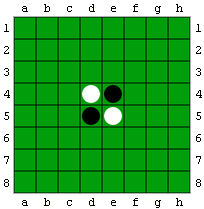
\includegraphics[height=4cm]{starting.png}
  \caption{Starting position}
  \label{fig:starting}
\end{figure}

\section{估值函数}
\label{sec:evaluator}

局面估值函数可以说是解决博弈问题中最重要的部分了,它决定了程序对局面的
评价,已经在选择对己方有利局面时的有效性。这里,约定对局面的估值越大,
意味着对黑方越有利;而对局面的估值越小,则意味着对白方越有利。

\paragraph{棋子计数}
这可能是最朴素的估值思想了,对棋局中黑白两色的棋子计数,若黑子个
数$B$多于白子个数$W$,则将棋子估值$p$定义为

\begin{equation}p = 100 \frac{B}{B+W}   \mathrm{ .}
\end{equation}

若白子个数多于黑子个数,则估值

\begin{equation}p = 100 \frac{W}{B+W}   \mathrm{ .}
\end{equation}

若$B = W$,则$p = 0$。

\paragraph{占角}
\emph{角(Corner)},如Figure \ref{fig:corner},位于棋盘
上a1、a8、h1和h8的位置。根据奕棋规则,角上的棋子是不能被翻转的,因此如
果一方占了一个角,它就一直是那一方的了。一旦一方占了一个角,可能许多子
受到角的保护,变成永远不会被翻转的棋子(即稳定子)。稳定子的数量能直接
影响到棋局的胜负,因此在对局中对角的抢占是极为重要的。

\begin{figure}[!hbp]
  \centering
  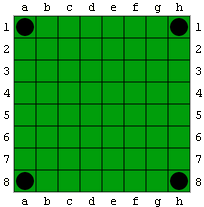
\includegraphics[height=4cm]{corner.png}
  \caption{Corner square}
  \label{fig:corner}
\end{figure}

记$B$为棋局中黑方占的角的个数,$W$为白方占的角的个数,则角估值$c$定义
为

\begin{equation}c = 25B - 25W   \mathrm{ .}
\end{equation}

\paragraph{临角}
根据前面的分析,由于角在黑白棋游戏中的重要性,对临近角的位置的防守也显
得尤为重要。在黑白棋术语中,将棋盘上b2、b7、g2和g7的位置称
为\emph{星位(X-square)},如Figure \ref{fig:x-square};将棋盘
上a2、a7、b1、b8、g1、g8、h2和h7的位置称
为\emph{C位(C-square)},如Figure \ref{fig:c-square}。星位通常会让对手占
去相邻的角,棋局早期下了X点几乎就等于放弃了与之相邻的角。

\begin{figure}[!htbp]
  \centering
  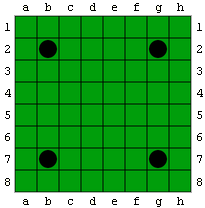
\includegraphics[height=4cm]{x-square.png}
  \caption{X-square}
  \label{fig:x-square}
\end{figure}

\begin{figure}[!htbp]
  \centering
  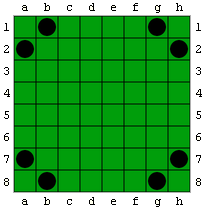
\includegraphics[height=4cm]{c-square.png}
  \caption{C-square}
  \label{fig:c-square}
\end{figure}

为了计算棋局的临角估值,记黑子所占的临角点数为$B$,白子所占的临角点数
为$W$,定义棋局的临角值$l$为

\begin{equation}l = -12.5B + -12.5W  \mathrm{ .}
\end{equation}

\paragraph{行动力}
\emph{行动力(Mobility)},指一方拥有的可选棋步数目,在实战上不包
括可选的坏棋(例如弃角或筑墙)。当可选棋步耗尽时,就表示失去了行动力。
保持己方行动力以及耗尽敌方行动力是棋局开局和中局的目标,拥有较多行动力
的一方通常较为优势。

\paragraph{边界}
\emph{边界(Frontier)},边缘子的集合,指的是与空格相邻的棋子个数。这些
棋子因为与空格相邻,很容易被对方在空格中放下一颗棋子而失去,因此应该尽
量减少己方的边界子数量。记黑方的临近空格的棋子个数为$B$,白方临近空格
的棋子个数未$W$。若$B>W$,定义边界估值$f$为

\begin{equation}f = -100 \frac{B}{B+W}   \mathrm{ .}
\end{equation}

\paragraph{位置估值}
这是根据棋盘上格子的重要性,对棋盘上每个格子赋的权值。由于棋盘是关于垂
直、水平两个轴对称的,因此这里只给出了左上角的权值,将它镜像翻转后就能
得到整张棋盘的权值。

\begin{equation}
 V =  \begin{pmatrix}
    20 & -3 & 11 & 8\\
    -3 & -7 & -4 & -1 \\
    11 & -4 & 2 & 2\\
    8 & 1 & 2 & -3 \end{pmatrix}
  \mathrm{ .}
\end{equation}

矩阵中给出的这些权值是根据实验得到的。

棋局的位置估值$d$是用矩阵中的权值的线性组合定义的,

\begin{equation}
  d = \sum_{i=1}^4\sum_{j=1}^4\sigma(i,j)V_{ij}
  \mathrm{ .}
\end{equation}

其中,$\sigma(i, j)$称为\emph{颜色系数(color coefficient)}

\begin{equation}
  \sigma(i, j)=\left\{
    \begin{array}{cl}
      -1 & \mathrm{if } V_{ij} \mathrm{ is white}\\
      0 & \mathrm{if } V_{ij} \mathrm{ is empty} \\
      1 & \mathrm{if } V_{ij} \mathrm{ is black}
    \end{array}
  \right.
  \mathrm{ .}
\end{equation}


特别的,这六种特征的估值都被标准化到区间$[-100, 100]$上。这让我能一致
化地处理这些特征,并给我在调整这些特征估值在最后的估值函数中的权重时带
来了方便,避免了特征中``自带''的权重。最后的总估值$S$的定义为

\begin{equation}
  S = \sum_{k=0}^nw_kc_k \mathrm{ ,}
\end{equation}

其中,$n$是特征编号,$c_i$是第$i$种特征,$w_i$是第$i$种特征值的权值,
权值是在实验中测定的。

最终,权值向量被确定为$(10, 901.724, 382.026, 78.922, 78.922, 74.396,
10)$.

\section{博弈搜索策略}
\label{sec:gaming}

在博弈问题中,虽然对局面的估值是核心,但还需要在博弈树上搜索得到最优策
略。这里介绍在课程设计中使用到的两种搜索策略。

\subsection{Minimax}
\label{sec:minimax}

Minimax策略是在博弈树的搜索中,最朴素的搜索策略。这里首先定
义\emph{Max局面}和\emph{Min局面}的概念。

\paragraph{Max局面} 假设当前局面轮到黑方走,有多种决策可以选择,其中每
种觉得都导致一种子局面(sub-state)。由于决策权在黑方手中,当然会选择估
价函数值$f$最大的子局面。因此,该局面的决策函数只等于子局面$f$只的最大
值,把这样的局面称为Max局面。


\paragraph{Min局面} 若当前局面轮到白方走,有多种决策可以选择,其中每种
觉得都导致一种子局面。但由于决策权在白方手中,当然会选择估价函数值$f$最
小的子局面。因此,该局面的决策函数只等于子局面$f$只的最小值,把这样的局
面称为Max局面。

因此,在搜索博弈树的过程中,我们如果能完全计算某个局面的所有子局面的估
价函数值,根据当前局面是Max或Min局面,返回相应的最大/最小值就可以实现选
择对己方最有利的策略。

但由于实际问题中,时间、空间都是受到限制的,而对于黑白棋这样的游戏,状
态空间是很大的。对于一个典型的中盘局面,每一步都有至少10种不同的可选策
略,这里我们把局面中可以选择的策略数称为局面的\emph{分支因子},那么仅仅
搜8步之后我们就临着$10^9$个待估价状态。因此穷举所有的子局面的策略是不可
取的。可以认为规定一个搜索的最大深度|depth|。若递归的深度达到|depth|则
直接返回当前局面的估价函数值。

\subsection{$\alpha\beta$剪枝}
\label{sec:alpha-beta}

如上一节中所说,状态空间的指数级增长使得我们不能在递归搜索的时候搜得太
深,但更深的搜索层数意味着对未来局面更好的把握。为了解决这个矛盾,必须
引入策略加速搜索。剪枝策略是一种常用的加速搜索的技术,这一节介绍一种名
为\emph{$\alpha\beta$剪枝}的剪枝策略。

在对博弈树进行递归搜索的时候,加上$\alpha$和$\beta$两个参数记录当前局
面之前搜索过的局面得到过的最好的上界和下界。



\section{GUI}
\label{sec:GUI}
这次的课设项目的GUI使用的是时下很流行的脚本语言Python。由于它的跨平台特
性和很好的GUI框架支持,借着这次数据结构课程设计的机会,我系统地学习了这
门语言。


\subsection{wxPython}
\label{sec:wxPython}

Python的GUI框架多种多样,有自带的Tk,还有PyQt、PyGTK、wxPython等不同的
框架,我这次使用的GUI框架是wxPython。

wxPython 是 wxWidget 的 Python 绑定,在Windows, Linux, Mac OS X等多种桌
面平台下都有原生实现。使用wxPython作为图形界面的框架,让程序自然地具有
了很好的跨平台特性。

但想要在Windows下使用,还是需要安装wxWidget的库。

\subsection{Python as a glue}
\label{sec:implementation}

在这次课程设计中,由于课程性质的要求(考察对数据结构的掌握)和语言效率
的考虑,AI部分的实现是使用的C语言编写的。由于GUI是使用Python开发的,不
能直接调用编译好的动态链接库。但这并不是一个不可解决的问题:Python 作为
一种脚本语言,在程序开发的过程中,往往起到了\emph{胶水(glue)}一般的作用,
将不同语言开发的库整合到一个项目中来。

Python的Dev包提供了可以供C语言调用的头文件,使得我们可以在C里使
用Python传来的参数,在Python里调用使用这些头文件开发的C程序。这使得
易于开发的Python程序也可以具有C程序的高效性。

\subsubsection{SWIG}
\label{sec:swig}
但是改用这些Python提供的库函数编写需要一段适应的时间,因此就有了SWIG这
样的项目。它能让开发者使用C中的数据类型和数组等开发,再加上一个\emph{接
  口文件}就可以编译出可供Python调用的库了。

接口文件里,分别描述了C语言编写的函数在接受Python调用时传递来的参数时应
该如何解析它,和C语言编写的函数在返回值时应该如何将它处理成Python的数据
类型。

在这次课程设计中,我使用SWIG编译了我的AI模块。这样,我的AI可以更高效地
工作。

\section{软件工程}
\label{sec:software_engineering}

在这次课程设计的开发过程中,我简单使用了软件工程中要求的两种方法:单元
测试和版本控制。

\subsection{单元测试}
\label{sec:unittest}
在开始编写Game类和AI模块前,我就编写了Game类和AI模块的相应单元测试。这
在软件开发中,叫做``测试驱动开发''。这样可以在开发时随时测试,保证开发
的过程中,不会因为功能的添加或修改导致新的BUG。

在这次的开发中,寻找可落子的点和翻转棋盘的点的功能出现过几次Bug,但我
写的单元测试都帮我第一时间发现了Bug,为我节约了不少时间。

这次使用的是随Python一起分发的unittest框架。这个框架下,可以方便地将测
试用例(Test Case)组织成测试套件(Test Suite)。可以把不同类型的测试组
织到不同的Test Suite中。比如我就将对Game类和AI模块的测试放到了两个不同
的文件中,便于管理。

对Game类的测试中,我测试了在棋盘4个角点、4条边上的点、不挨着任何边的点,
和从8个方向挨着黑子和白子的点的共20多个测试点。

对AI模块的测试相对简单一些,因为AI搜索的量太大,难以通过手动模拟找到最
优的策略。

下面的运行单元测试的结果,可以看到我的代码通过了所有的测试。

\begin{verbatim}
...
---------------------------------------------------------
Ran 25 tests in 0.263s

OK
\end{verbatim}


\subsection{版本控制}
\label{sec:revision-control}

版本控制(Revision control)是维护工程蓝图的标准作法,能追踪工程蓝图从
诞生一直到定案的过程。此外,版本控制也是一种软件工程技巧,借此能在软件
开发的过程中,确保由不同人所编辑的同一程式档案都得到同步。

在这次的课程设计中,版本控制系统帮我避免了因为在调试寻找可用点功能时添
加的调试代码对主分支的影响。而且在开发Hash功能时,我开辟了一
个``Hash''分支,避免了对搜索剪枝功能的开发进度的影响。

\begin{lstlisting}[caption={pyiagno.py}]
#!/usr/bin/python

import wx
from frame import IagnoFrame

class IagnoApp(wx.App):
    def OnInit(self):
        self.frame = IagnoFrame(None, -1, "PyIango")
        self.SetTopWindow(self.frame)
        self.frame.Show()
        return 1

# end of class MyApp

if __name__ == "__main__":
    app = IagnoApp(0)
    app.MainLoop()
\end{lstlisting}

\begin{lstlisting}[caption={frame.py}]
#!/usr/bin/python

import wx
from game import IagnoGame
from ai import *

class IagnoFrame(wx.Frame):

    # Player movement instructions
    PlayerStr = ("Dark's move", "Light's move")

    # =======================================================
    # Constructor
    # =======================================================
    def __init__(self, *args, **kwds):
        kwds["style"] = wx.DEFAULT_FRAME_STYLE ^ (wx.RESIZE_BORDER
                                                  | wx.MINIMIZE_BOX
                                                  | wx.MAXIMIZE_BOX)
        wx.Frame.__init__(self, *args, **kwds)
        self.frame_statusbar = self.CreateStatusBar(2, 0)

        self.Bitmaps = [wx.Bitmap("image/dark.png", wx.BITMAP_TYPE_ANY),
                        wx.Bitmap("image/light.png", wx.BITMAP_TYPE_ANY),
                        wx.Bitmap("image/blank.png", wx.BITMAP_TYPE_ANY)]

        
        self.Bind(wx.EVT_PAINT, self.OnPaint)
        self.Bind(wx.EVT_LEFT_UP, self.OnClick)
        
        self.Game = IagnoGame(ai=insane_ai)
        # self.Game = IagnoGame(ai=None)
        self.__set_properties()


    def __set_properties(self):
        self.SetTitle("PyIango")
        self.SetSize((320, 346))
        self.frame_statusbar.SetStatusWidths([-4, -6])
        self.frame_statusbar.SetStatusText(IagnoFrame.PlayerStr[self.Game.Player], 0)
        self.frame_statusbar.SetStatusText("Dard: %d Light: %d" % (self.Game.DarkCnt, self.Game.LightCnt), 1)

    def __Draw(self, color, pos):
        x, y = pos
        dc = wx.ClientDC(self)
        dc.DrawBitmap(self.Bitmaps[color], x*40, y*40, True)
        
    def __AIMove(self, aiPlayer):
        while not self.Game.IsEnd and self.Game.Player == aiPlayer:
            x, y = self.Game.ai(self.Game.Board, aiPlayer, len(self.Game))
            try:
                l = self.Game.Set((x, y))
            except self.Game.InvalidPositionException:
                self.frame_statusbar.SetStatusText('Invalid move.', 0)
                raise 'AI Error'
            else:
                for yy, xx in l:
                    self.__Draw(aiPlayer, (xx, yy))
                self.__Update()
                
    def __Update(self):
        if self.Game.IsEnd:
            if self.Game.DarkCnt > self.Game.LightCnt:
                self.frame_statusbar.SetStatusText('Dark wins!', 0)
            elif self.Game.DarkCnt < self.Game.LightCnt:
                self.frame_statusbar.SetStatusText('Light wins!', 0)
            else:
                self.frame_statusbar.SetStatusText('Draw...', 0)
        else:
            self.frame_statusbar.SetStatusText(IagnoFrame.PlayerStr[self.Game.Player], 0)
        self.frame_statusbar.SetStatusText("Dard: %d Light: %d" % (self.Game.DarkCnt, self.Game.LightCnt), 1)

    # =======================================================
    # Event handlers
    # =======================================================
    def OnClick(self, evt):
        y, x = evt.GetPosition()

        player = self.Game.Player
        try:
            l = self.Game.Set((x/40, y/40))
        except self.Game.InvalidPositionException:
            self.frame_statusbar.SetStatusText('Invalid move.', 0)
        else:
            for yy, xx in l:
                self.__Draw(player, (xx, yy))
            self.__Update()

            # if is human-AI game
            if not self.Game.IsEnd and self.Game.ai:
                self.__AIMove(not player)

    def OnPaint(self, evt):
        sz = (40, 40)
        MemDC = [wx.MemoryDC(), wx.MemoryDC(), wx.MemoryDC()]
        map(lambda dc, bmp: dc.SelectObject(bmp), MemDC, self.Bitmaps)

        dc = wx.PaintDC(self)
        for i in range(8):
            for j in range(8):
                dc.DrawBitmap(self.Bitmaps[self.Game[i][j]], j*sz[0], i*sz[1], True)
                

# end of class IagnoFrame
\end{lstlisting}


\begin{lstlisting}[caption={game.py}]
#!/usr/bin/python

import copy
import pprint

class IagnoGame(object):
    """
    Implements the Reversi game.
    """
    
    # Enumerator of colors on board
    BRD_BLANK, BRD_DARK, BRD_LIGHT = range(-1, 2)

    # Directions to move
    __dir = ((-1, -1), (-1, 0), (-1, 1), (0, -1), (0, 1),
             (1, -1), (1, 0), (1, 1))

    # =======================================================
    # Exceptions
    # =======================================================
    class NotFoundException(Exception): pass
    class InvalidPositionException(Exception): pass

    # =======================================================
    # Constructor
    # =======================================================
    def __init__(self,
                 ai = None,
                 init = [[-1, -1, -1, -1, -1, -1, -1, -1],
                         [-1, -1, -1, -1, -1, -1, -1, -1],
                         [-1, -1, -1, -1, -1, -1, -1, -1],
                         [-1, -1, -1,  1,  0, -1, -1, -1],
                         [-1, -1, -1,  0,  1, -1, -1, -1],
                         [-1, -1, -1, -1, -1, -1, -1, -1],
                         [-1, -1, -1, -1, -1, -1, -1, -1],
                         [-1, -1, -1, -1, -1, -1, -1, -1]],
                 l = 0,
                 player = 0):
        """
        Initialize a new game.
        param init: the initial outline of the game.
        """
        self.__Board = copy.deepcopy(init) # set the initial board
        
        self.__Len = l                 # steps been taken

        self.__Valid = []              # valid place to set
        self.__Valid.append([])
        self.__Valid.append([])
        
        self.__Player = player         # initial player
        self.__End = False

        self.__DarkCnt = 0
        self.__LightCnt = 0

        self.ai = ai

        self.__Maintain()

    # =======================================================
    # Public methods
    # =======================================================
    def Set(self, pos):
        """
        Sets a piece at pos for player.
        Returns the changed grids.
        If pos is not valid for player, raises InvalidPositionException.
        """
        player = self.__Player
        if pos in self.Valid[player]:
            self.__Output('Step: %d, Player: %s, (%d, %d)' % (len(self)+1, ('Dark', 'Light')[player], pos[0], pos[1]))
            x, y = pos
            self.__Board[x][y] = player
            self.__Len += 1
            self.__Player = int(not self.__Player)
            return self.__Update(pos)
        else:
            raise self.InvalidPositionException
        

    # =======================================================
    # Overloaded methods
    # =======================================================
    def __getattr__(self, attrname):
        if attrname == 'Player':
            return self.__Player
        elif attrname == 'Valid':
            return tuple(copy.deepcopy(self.__Valid))
        elif attrname == 'IsEnd':
            return self.__End
        elif attrname == 'Board':
            return copy.deepcopy(self.__Board)
        elif attrname == 'DarkCnt':
            return self.__DarkCnt
        elif attrname == 'LightCnt':
            return self.__LightCnt
        else:
            raise AttributeError, attrname
        
    def __len__(self):
        """
        The length of a game is the current number of steps
        """
        return self.__Len

    def __getitem__(self, idx):
        """
        Access to the board by index
        """
        return self.__Board[idx][:]


    # =======================================================
    # Private methods
    # =======================================================
    def __Update(self, pos):
        """
        Update the board, after put a piece on pos.
        Returns a tuple containing the positions that was updated.
        """
        x, y = pos
        player = self[x][y]
        ret = [pos]
        for d in self.__dir:
            try:
                li = self.__Find(player, pos, d)
            except:
                pass
            else:
                for x, y in li:
                    self.__Board[x][y] = int(not self.__Board[x][y])
                ret += li
        self.__Maintain()
        return tuple(ret)

    def __Find(self, color, pos, d):
        """
        Find the consecutive grids which have different color with the color of pos in direction d.
        Returns the tuple of founded positons.
        If not found, raises NotFoundException.
        """
        x, y = pos
        dx, dy = d
        ret = []
        x += dx
        y += dy
        while x in range(8) and y in range(8) and self[x][y] == (not color):
            ret.append((x, y))
            x += dx
            y += dy
            
        if x in range(8) and y in range(8) and self[x][y] == color and ret != []:
            return tuple(ret)
        raise self.NotFoundException

    def __Maintain(self):
        """
        Maintains the valid positions and pieces count for each
        player.
        """
        self.__Valid[0] = []
        self.__Valid[1] = []
        self.__LightCnt = 0
        self.__DarkCnt = 0
        
        for (x, line) in enumerate(self):
            for (y, piece) in enumerate(line):
                pos = (x, y)
                if piece == IagnoGame.BRD_BLANK:   # check valid pos
                    for color in range(2):
                        for d in self.__dir:
                            try:
                                self.__Find(color, pos, d)
                            except:
                                pass
                            else:
                                self.__Valid[color].append(pos)
                                break
                elif piece == IagnoGame.BRD_LIGHT:  # count pieces
                    self.__LightCnt += 1
                elif piece == IagnoGame.BRD_DARK:
                    self.__DarkCnt += 1
        print self.Valid[0]
        print self.Valid[1]
        if self.Valid[self.__Player] == []:
            self.__Player = int(not self.__Player)
                
        if self.Valid[0] == [] and self.Valid[1] == []:
            self.__End = True

    # =======================================================
    # For debug only
    # =======================================================
    def __Output(self, msg=''):
        """
        For debug only, print the current board.
        """
        print 'PyIagno Debug:'
        print msg
        pprint.PrettyPrinter().pprint(self.Board)

# end of class IagnoGame
\end{lstlisting}

\begin{lstlisting}[language=make, caption=Makefile]
PYLIB = /usr/bin
PYINC = /usr/include/python2.6
CLIB  = ai_src
PHONY = clean

# the library plus its wrapper
_ai.so: $(CLIB)/ai_wrap.o $(CLIB)/ai.o
	gcc -shared $(CLIB)/ai_wrap.o $(CLIB)/ai.o -L$(PYLIB) -lpython2.6 -o $@


# generated wrapper module code
$(CLIB)/ai_wrap.o: $(CLIB)/ai_wrap.c $(CLIB)/ai.h
	gcc $(CLIB)/ai_wrap.c -g -I$(CLIB) -I$(PYINC) -c -o $@

$(CLIB)/ai_wrap.c: $(CLIB)/ai.i
	swig -python -I$(CLIB) -outdir $(CLIB)/ $(CLIB)/ai.i
	mv $(CLIB)/ai.py .

# C library code (in another directory)
$(CLIB)/ai.o: $(CLIB)/ai.c $(CLIB)/ai.h
	gcc $(CLIB)/ai.c -g -I$(CLIB) -c -o $(CLIB)/ai.o

clean:
	rm -f *.so *.o *.pyc ai.py $(CLIB)/*.o $(CLIB)/*.pyc $(CLIB)/ai_wrap.c 
\end{lstlisting}

\end{document}

%%% Local Variables: 
%%% mode: latex
%%% TeX-master: t
%%% End: 
